%!TEX root = ../report_template.tex
\section*{Methods}
%Todo: Think about citations



\textbf{The Pearson correlation coefficient} \cite{rodgers_thirteen_1988}, denoted as $r$, is a statistical measure used to assess the linear relationship between two sets of data, $X$ and $Y$. It is computed as the ratio of the sample covariance of the $X$ and $Y$ to the product of their sample standard deviations:
\begin{equation}
    r = \frac{\sum_{i=1}^n (X_i - \overline{X}) (Y_i - \overline{Y})}{\sqrt{\sum_{i=1}^n(X_i-\overline{X})^2 \cdot \sum_{i=1}^n(Y_i-\overline{Y})^2}}
\end{equation}


\paragraph{Datasets:}
The datasets used in this paper can be grouped into causes and effects. Therefore, the causes are societal, demographic, or political factors influencing the quality of the German school system. This could be the number of students, teachers, or budget provided by the German government. In contrast, this paper defines the effects of the causes as observable measures of the students' performance. Examples are the average grades, PISA study results, or the rate of repeaters and school-leavers.

% Causes
The first cause dataset is provided in the \textit{Fachreport Schuljahr 2020/21} of the \citeauthor{statistische_bundesamt_allgemeinbildende_2022} and contains the number of teachers from 1992 until 2020. The dataset groups them primarily according to their contract type, federal state, and school type. This paper merges the teacher counts with two student datasets, which are published in the \textit{Genesis} database of the \citeauthor{statistische_bundesamt_statistisches_2023}. Both provide the number of children as different groupings and aggregations. The first contains the number of children per grade and school type  for the years 1998 to 2022. In contrast, the second table provides the absolute amount of children, leavers, and beginners in each federal state from 1997 to 2022. Therefore, the analysis of the merged dataset can only be conducted separately for school types and federal states.

To conclude the causes, this paper introduces the budget per child, which is provided in the \textit{Genesis} database of the \citeauthor{statistische_bundesamt_statistisches_2023}. The dataset contains the budget per child for the years 2010 to 2022 and is grouped by federal states. In contrast to the demographic and societal causes above, the budget models a direct political factor. To adjust the budget to inflation, it is multiplied with the \textit{Verbraucherpreisindex} relative to 2022 provided by the \citeauthor{statistische_bundesamt_statistisches_2023}. 


% Effects
Moreover, the primary effects on students' performance are the basis for the analysis of the German school system. One of the few publicly available datasets containing grades is the average Abitur grades per federal state. The grades are published every year by the \citeauthor{kultusminister_konferenz_abiturnoten_nodate}. Each file contains the count of children per written grade and federal state. In addition, the grades are defined in $0.1$ steps, with $4.0$ as the worst and $1.0$ as the best grade. Furthermore, the amount of children who failed with a grade worse than $4.0$ is aggregated in an additional column. 

Although this is a great model for the performance of children attending grammar schools, a general performance measure for all school types is required. Accordingly, this paper uses the number of repeaters derived from the \textit{{GENESIS}} Database of the \citeauthor{statistische_bundesamt_statistisches_2023}. There, the absolute count of repeaters by federal state, school type, and year is provided for the years 1998 to 2022.

\paragraph{Figures}

\begin{figure}[h]
    \centering
    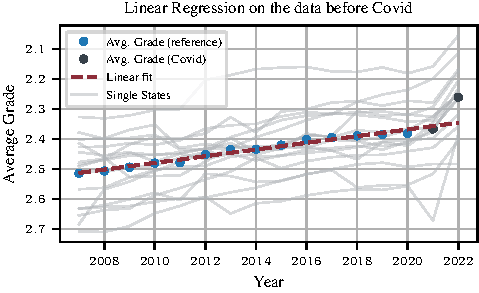
\includegraphics{fig/fig_rising_grades.pdf}
    \caption{Average Abitur grades before (\textcolor{TUlightblue}{\tikz\draw[fill={TUlightblue}] (0,0) circle (0.25em);}) and after the COVID-19 pandemic (\textcolor{TUdark}{\tikz\draw[fill={TUdark}] (0,0) circle (0.25em);}) with a linear regression line (\textcolor{TUred}{\rule[-0.2ex]{0.5em}{2pt} \rule[-0.2ex]{0.5em}{2pt}}) of the years 2007 to 2020. In the background the figure contains average grades foreach federal state (\textcolor{TUgray}{\rule[-0.2ex]{0.5em}{1pt}}).}
    \label{fig:rising-grades}
\end{figure}

%TODO: Better beginning
\autoref{fig:heatmap_correlation_students_per_teacher_repeaters_budget} presents a visualization of the Pearson correlation coefficients, analyzing the relationship between the number of children per teacher and the average number of repeaters, as well as the educational budget per state. 

%TODO: Reformulate
Initially, to compute the relative number of repeaters, the \textit{Number of Repeaters} dataset is merged with the \textit{school-children-by-state} dataset, grouped by \textit{Federal State} and \textit{Year} and the number of repeaters is divided by the total number of school children. Subsequently this dataset is merged with the \textit{budget} and the \textit{students by teacher} dataset, using \textit{Federal States} and \textit{Years} as the common attributes for alignment. 

Finally, for each state, the Pearson correlation coefficient is calculated across different years to ascertain the correlation between the students-to-teacher ratio and the budget, as well as the average amount of repeaters.

In order to visualize the data over the states a heatmap for the german federal states is created. Therefor the Pearson correlation coefficients are normalized to the used colormap scale. Each state receives the appropriate computed color then.

\begin{figure}[h]
    \centering
    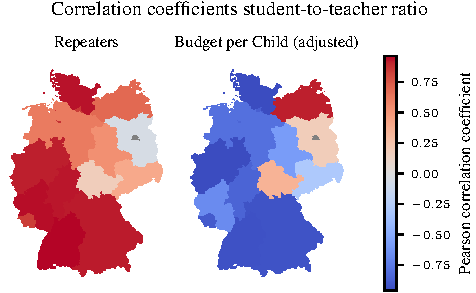
\includegraphics{fig/fig_heatmap_correlation_students_per_teacher_repeaters_budget.pdf}
    \caption{Pearson correlation coefficients between the student-to-teacher ratio and the relative repeater count (left) and the inflation-adjusted average budget per child (right). \textcolor{red}{Red} indicates positive, \textcolor{gray}{gray} neutral, and \textcolor{blue}{blue} negative correlations between the variables.}
    \label{fig:heatmap_correlation_students_per_teacher_repeaters_budget}
\end{figure}
